\documentclass{article}
\usepackage{amsmath}
\usepackage{graphicx}
\graphicspath{ {./images/} }
\usepackage[title]{appendix}
%\usepackage{nips_2018}
\usepackage[a4paper, total={7in, 10in}]{geometry}


\begin{document}
	\title{Solving differential equation by Neural Network}
	\maketitle
We formulate ordinary differential equation(ODE) and partial differential equation(PDE) as learning algorithm for neural network. The neural network is trained to satisfy the differential operator and boundary conditions using stochastic gradient descent. 

\tableofcontents
\section{Experiment}
This section presents the detail of implementation and the accuracy of empirical result for numerical examples.

\subsection{Examples for ODE}
\textbf{Problem 1.1}
Given $x_i \in [0,1]$, $1 \leq i \leq N$ where i is the number of discretization points. We would like to find the solution of $\Psi(x)$ for the following equation.   
\[\frac{d}{dx}\Psi + (x+\frac{1+3x^2}{1+x+x^3})\Psi = x^3 +2x +x^{2}\frac{1+3x^2}{1+x+x^3}\]
with $IC =\Psi (0)$  and $BC = \Psi(N)$. 
The analytic solution is 
\[\Psi_{a}(x)=\frac{e ^{-x^2/2}}{1+x+x^3} + x^2\] 
In consideration of (\ref{eq:trial_sol_ode1}) below, the form of trial solution is taken to be: 
\[\Psi_t(x) = \Psi(0) + xO(x,p)\] with $IC =\Psi(0)$ and $BC=\Psi(1)$.
We look for the solution $\Psi_t$ by minimizing the following error quantity:
\[E_\text{error} =  \sum_{i} (\frac{d \Psi_{t}(x_i)}{dx}-f(x_i,\Psi_{t}(x_i)))^2\]
where
\[f(x_i,\Psi_{t}(x_i)) =x^3 +2x +x^{2}\frac{1+3x^2}{1+x+x^3} - (x+\frac{1+3x^2}{1+x+x^3}\Psi)\]

\medskip\noindent
In each iteration, we update the weight to be

\begin{equation}
\begin{aligned}
	w_{ij}^{(r+1)} = w_{ij}^{(r)} - \gamma_{r}*\frac{\partial E_\text{error}}{\partial w_{ij}} \\
	v_{j}^{(r+1)} = v_{j}^{(r)} - \gamma_{r}*\frac{\partial E_\text{error}}{\partial v_{j}}
\end{aligned}
\end{equation}

where $\gamma_r$ is the learning rate. 

\medskip \noindent
Figure \ref{fig:trial_ode1} displays the actual and computed solution of $\Psi_{t}(x_i)$ at the grid points.
\begin{figure}
	\centering
	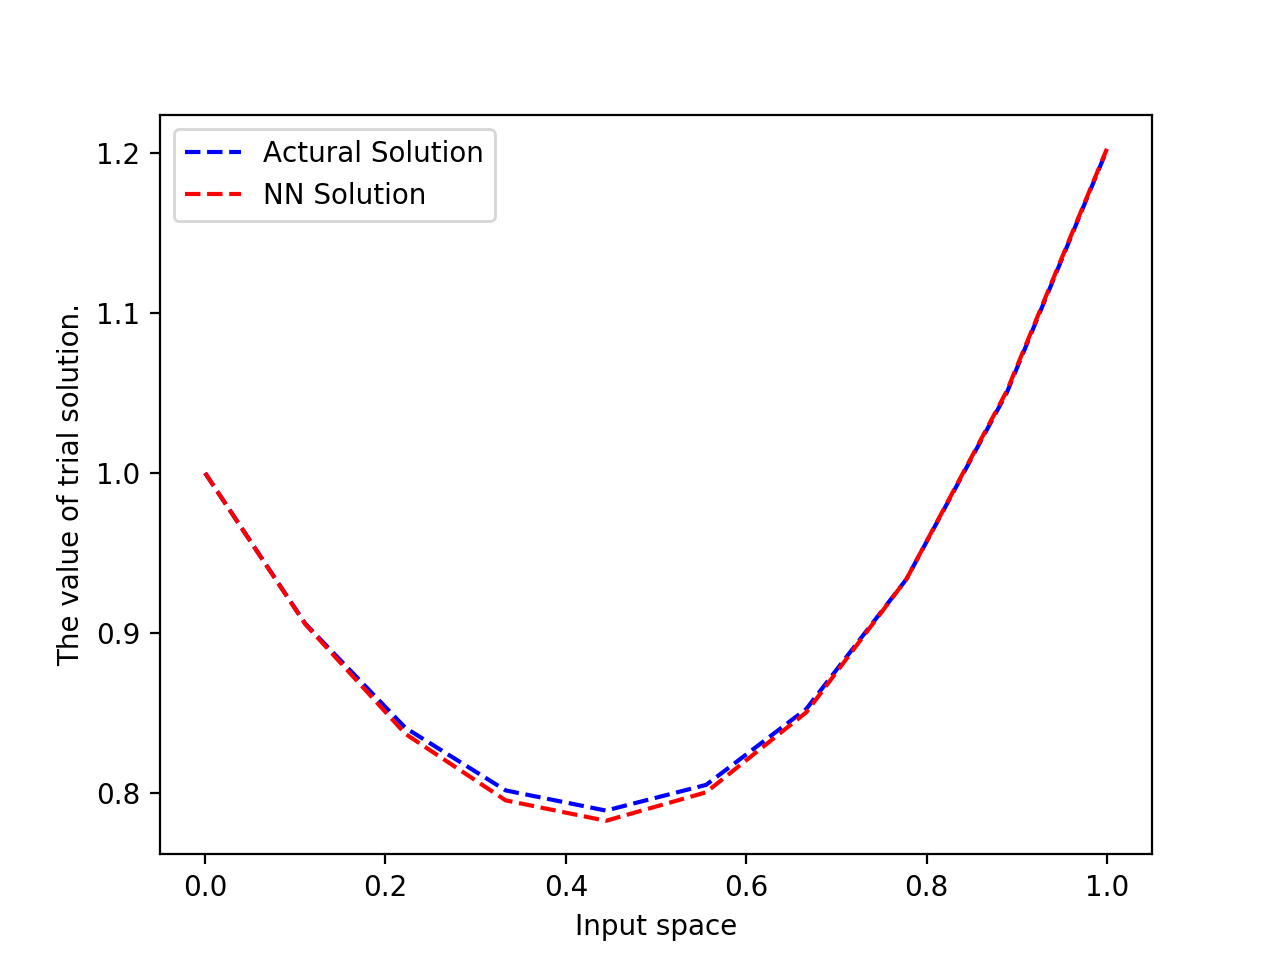
\includegraphics[width=0.5\textwidth]{ode_1.png}
	\caption{The actual and computed solution in problem 1.1. }
	\label{fig:trial_ode1}
\end{figure}

\medskip \noindent
\textbf{Problem 1.2} Given $x_i \in [0,2]$, $1 \leq i \leq N$ where i is the number of discretization points. We would like to find the solution of $\Psi(x)$ for the following equation.   

\[\frac{d}{dx} \Psi + \frac{1}{5} \Psi = e^{\frac{x}{5}}cos(x)\]

\medskip \noindent
The analytic solution is:
\[\Psi_{a}(x) = e^{\frac{1}{5}}sin(x) \]
In consideration of (\ref{eq:trial_sol_ode1}) below, the form of trial solution is taken to be: 
\[\Psi_t(x) = \Psi(0) + xO(x,p)\] with $IC = \Psi(0)=0$ and $BC =\Psi(N)$.

\medspace \noindent
Figure \ref{fig:trial_ode2} displays the actual and computed solution of $\Psi _t(x_i)$ corresponding to the domain. 

\begin{figure}
	\centering
	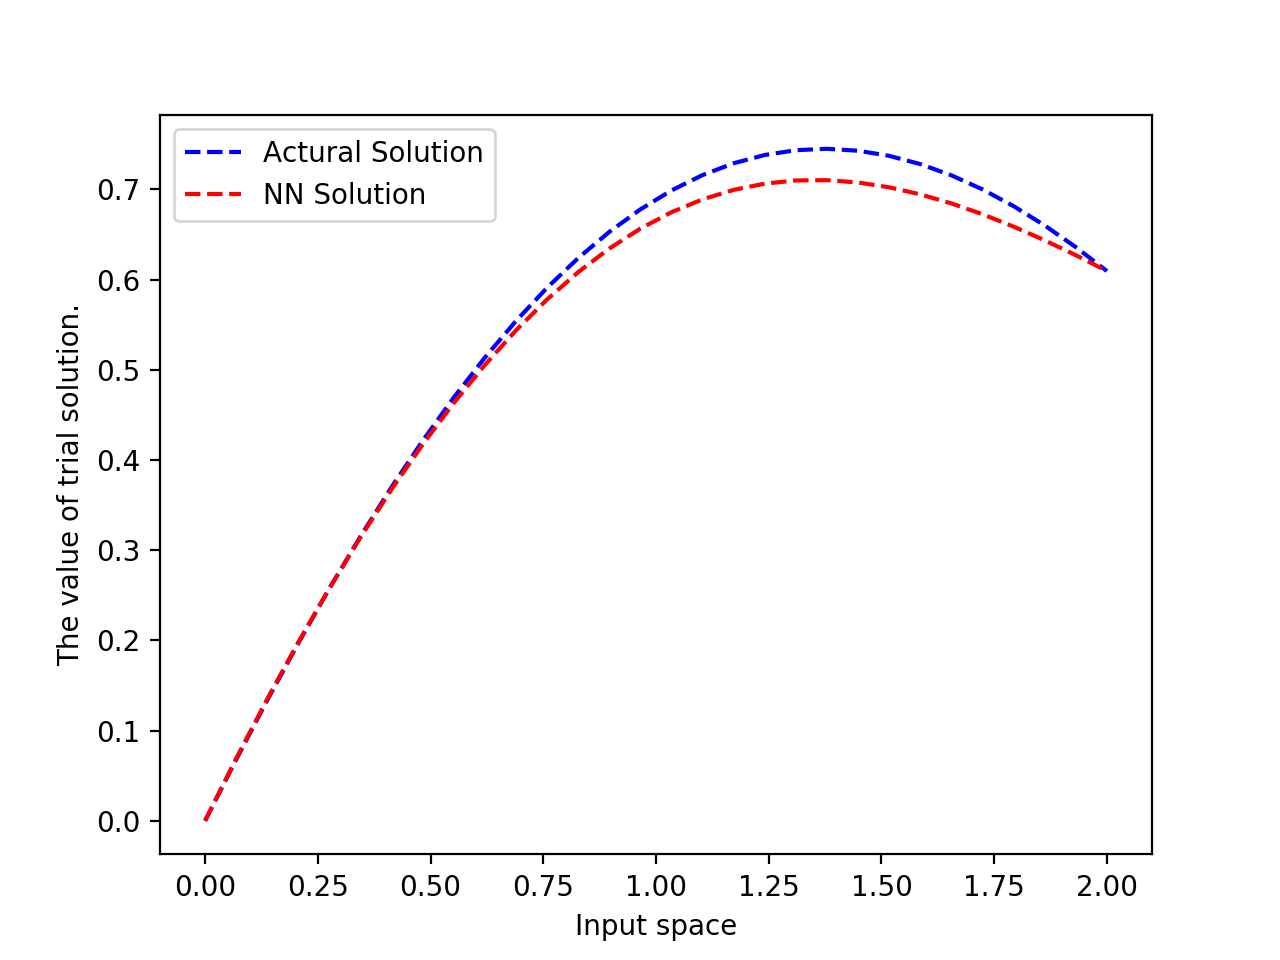
\includegraphics[width=0.5\textwidth]{ode_2.png}
	\caption{The actual and computed solution in problem 1.2. }
	\label{fig:trial_ode2}
\end{figure}

\medskip \noindent
\textbf{Problem 1.3} Given $x_i \in [0,2]$, $1 \leq i \leq N$ where i is the number of discretization points. We would like to find the solution of $\Psi(x)$ for the following equation.

\[\frac{d^2}{dx^2} \Psi + \frac{1}{5} \frac{d}{dx} \Psi + \Psi= -\frac{1}{5}e^{\frac{x}{5}}cos(x)\]

\medskip \noindent
The analytic solution is:
\[\Psi_{a}(x) = e^{\frac{1}{5}}sin(x) \]
In consideration of (\ref{eq:trial_sol_ode1}) below, the form of trial solution is taken to be: 
\[\Psi_t(x) = \Psi(0)(1-x)+ \Psi(1)x+x(1-x)O(x,p)\] with $IC = \Psi(0)=0$ and $BC =\Psi(N)$.

\medspace \noindent
Figure \ref{fig:trial_ode3} displays the actual and computed solution of $\Psi _t(x_i)$ corresponding to the domain. 

\begin{figure}
	\centering
	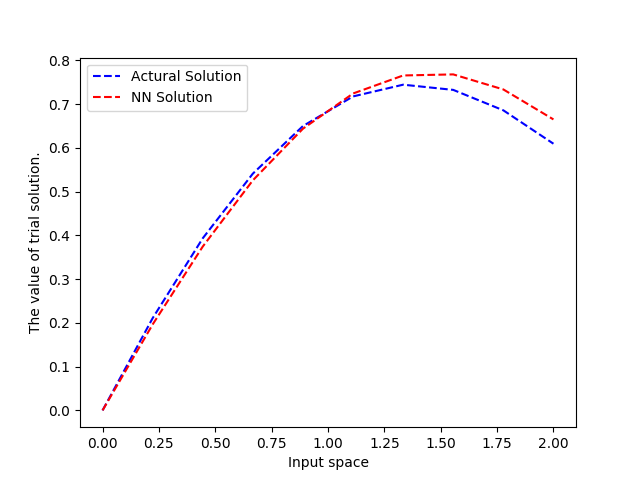
\includegraphics[width=0.5\textwidth]{ode_3.png}
	\caption{The actual and computed solution in problem 1.3. }
	\label{fig:trial_ode3}
\end{figure}

\section{Schematic of the Algorithm}

To make the differential equation solvable by NN, the trial solution and original equation have to be transformed into the specific form.  
Therefore, this section provides the formulation for differential equation to adjust in order to solve by NN.  
The approach is based on Lagaris\cite{lagaris} and  Chiaramonte\cite{chiaramonte}.

\subsection{Formulation}
 
The proposed approach is illustrated in terms of the following general differential equation:
\begin{equation}\label{eq:original_error}
G(x,\Psi (x),\bigtriangledown \Psi (x), \bigtriangledown \Psi (x)^2) = 0, x \in D
\end{equation}
\medskip \noindent
subject to certain boundary conditions (B.Cs),  where $x=(x_1, \dots , x_n) \in \mathbf{R}^n, D \subset \mathbf{R}$ and $\Psi$ is the trial solution employs a neural network and $D$ denotes the definition of domain. 
\begin{equation}\label{eq:trial_solution}
\Psi_{t}(x,p) = \hat{\Psi}(x) + F(x)N(x,p)
\end{equation}
The parameter $p$ is adjusted based on the weights and bias of neural network. 
$\hat{\Psi}(x)$ is the initial conditions(I.C.) which is set to be $\hat{\Psi}(0) = \Psi (0) =0$ and contains no adjustable parameters.
The scalar-value function $F(x)$ is chosen so as not to contribute to BC. 
$N(x,p)$ is the single-output forward neural network(NN).  
In order to be solved by NN, we transform (\ref{eq:original_error}) to the  following system of equations:
%\begin{equation}\label{eq:3}
%G(x_i,\Psi (x_i),\bigtriangledown \Psi (x_i), \bigtriangledown \Psi (x_i)^2) = 0, \forall %x_i \in D, \forall i = 1 \dots m
%\end{equation}
\begin{equation}\label{eq:total_error_sum}
E_{\text{error}}(p) = \min \sum_{i=1}^{m} G(x_i,\Psi (x_i),\bigtriangledown \Psi (x_i), \bigtriangledown \Psi (x_i)^2) ^2, \forall x_i \in D, \forall i = 1 \dots N
\end{equation}
subject to the constraints imposed by the B.Cs.
If $\Psi_{t}(x,p)$ denotes the trial solution, $\Psi_{t}(x,p)$ will minimize the related error of (\ref{eq:total_error_sum}). The general form of the trial solution $\Psi _t$ for the first order ODE can be written as:
\begin{equation}\label{eq:trial_sol_ode1}
\Psi_{t} (x_i) = \Psi(0) + x_iO(x_i,p) \forall x_i \in D, \forall i = 1 \dots N
\end{equation} 

%\medskip \noindent
%\textbf{Below is the outline of the NN for solving ODE: }
%\begin{itemize}
%	\item Input $x_i$: The number of equidistant points for (\ref{eq:total_error_sum}) in $x\in D, \forall i = 1 \dots N$. For example, if the $D={x^{(i)} \in D; i = 1, \dots , 10}$, the $E_{\text{error}}$ is trained by discretizing  $10$ equidistant points in $[0,1]$. 
%	\item Hidden layer $h$: Each unit in the layer corresponds to the discrete time step with sigmoid activation function in (\ref{eq:activation}). 
%	\item Output $O_i$: The output is used to measure the trial solution in (\ref{eq:forward_output}).   
%\end{itemize}


\section{Stochastic Gradient Descent}
Lagaris\cite{lagaris} had proved that Broyden–Fletcher–Goldfarb–Shanno (BFGS) algorithm method is quadraticly convergent and has demonstrated excellent performance at computing the gradient of the error. 
Therefore, quasi-Newton BFGS algorithm was used to minimize the loss function in our model.



\subsection{ODE}
\subsubsection{First Order ODE}
We consider the first order ODE:
\[\frac{d}{dx}\Psi(x)=f(x,\Psi)\]
We discretinize our domain $[0,1]$ into n grids and obtain input vector $x_i$, $1 \leq i \leq N$ where i denotes the single input unit in discretenized domain.
We apply activation function to obtain the output of hidden unit. A popular choice for choosing activation function is the sigmoid function. 
\begin{equation}\label{eq:sigmoid}
\sigma(y) = \frac{1}{1+e^{y}} 
\end{equation}
The output of hidden units given by activation function is mapped from 0 to 1.
\begin{equation}\label{eq:hidden_unit}
H_{h} = \sum_{i=1}^{n=N} \sigma (w_{ih}*x_i)
\end{equation}

\medspace \noindent
The output forward propogation of NN is:
\begin{equation}\label{eq:output_ode}
O = \sum_{i=1}^{N} \sum_{h=1}^{H} \textit{v}_{j}\sigma (w_{ih}x_{i}) + u_i
\end{equation}
\medspace \noindent
Figure \ref{fig:nn_struct} expresses the diagram of NN with one hidden layer looking for the parameters for trial solution in ode and pde. This example only has one hidden layer. After we get the output for whole $x_{i}$, $i \in \{0, \dots , n\}$ via NN, we obtain the sum of error quantity. 

\begin{figure}
	\centering
	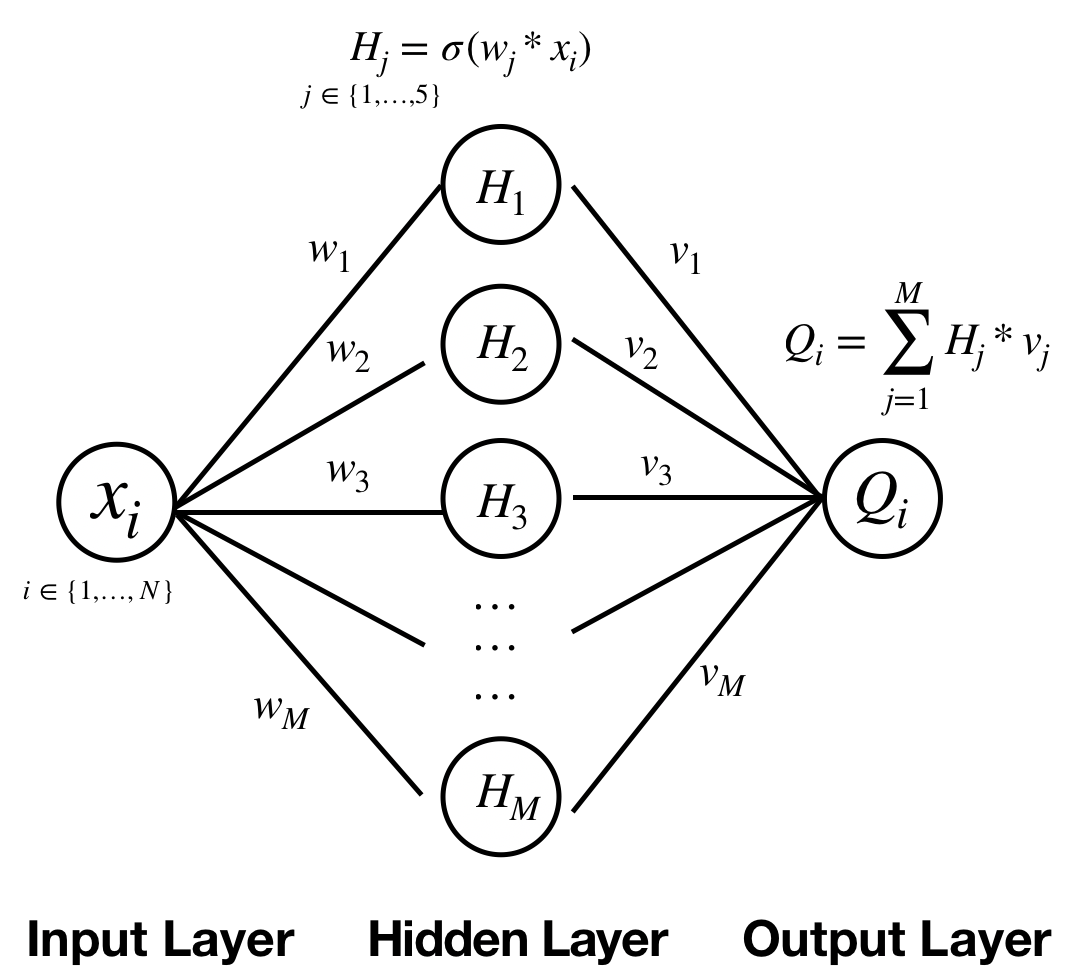
\includegraphics[width=0.4\textwidth]{nn_struct.png}
	\caption{The diagram of Neural Network for computing the parameters of trial solution in ode $O_{i}(x_i,p)$ with one hidden layer. }
	\label{fig:nn_struct}
\end{figure}

\begin{equation}\label{eq:total_error_ode}
\begin{aligned}
E &= E_i[p] + \dots + E_{n}[p] \\
E_\text{i}[p] &=\sum_{i=1}^{N} \{ \frac{d \Psi_{t}(x_i)}{dx}-f(x_{i}, \Psi_{t}(x_i))\}^{2} 
\end{aligned}
\end{equation}

\medskip \noindent
where p is the parameters in NN and $f(x_i,\Psi_{t}(x_i))$ is the value of $\frac{d}{dx}\Psi$. 
In the case of one dimension ode, we obtain the value after we shift all the items except for $\frac{d}{dx}\Psi$ to the right side. 

\medskip \noindent
We optimize the parameters of NN by minimizing the total error quantity in (\ref{eq:total_error_ode}) from $E_i, i \in \{1 \dots n\}, h \in \{1 \dots H\}$. 
\begin{equation}\label{eq:weight_ode_v}
\frac{\partial E}{\partial v_{h}} = \sum_{i=1}^{N} \frac{\partial E_\text{i}}{\partial O_i} \frac{\partial O_i}{\partial v_{h}} 
\end{equation}
\begin{equation}\label{eq:weight_ode_w}
\frac{\partial E}{\partial w_{ih}} = \sum_{i=1}^{N} \frac{\partial E_\text{i}}{\partial O_i} \frac{\partial O_i}{\partial w_{ih}} 
\end{equation}
where h is the number of hidden unit in each hidden layer, $1 \leq h \leq H$

\begin{equation}\label{eq:weight_ode_Ev}
\frac{\partial E_{i}}{\partial O_i} = 2(\{\frac{\partial \Psi_{t}(x_i)}{\partial x}-f(x_{i}, \Psi_{t}(x_i))\})
\end{equation}
\medskip \noindent
To calculate the (\ref{eq:weight_ode_Ev}). We need to differentiate the trial solution $\Psi_{t}(x_i)$:
\begin{equation}\label{eq: ode_trial_x}
\frac{\partial \Psi_{t} }{\partial x} = \frac{d \Psi (0)}{dx} + \frac{d}{dx}O_{i}(x_1,p) + x\frac{d O_{i}(x_1,p)}{dx}
\end{equation}
These equations reduce to 
\begin{equation}\label{eq:x_ode_Psix}
\frac{\partial \Psi_{t} }{\partial x} = O_{i}(x,p) + \sum_{i=1}^{N}\sum_{h=1}^{H} \textit{v}_{h} w_{ih} \sigma (w_{ih}x_{i})_{h} 
\end{equation}
Using (\ref{eq:x_ode_Psix}) and $f(x_{i}, \Psi_{t}(x_i))$, the gradient of $O_i$ is:
\begin{equation}\label{eq:partial_NV}
\frac{\partial O_i}{\partial v_{h}} = \sum_{h}^{H} \sum_{i=1}^{N}\sigma (w_{ih}x_{i})
\end{equation}
\medspace \noindent
We compute the gradient of $E_i$ with respect to input to hidden weight by using (\ref{eq:weight_ode_v})-(\ref{eq:partial_NV}) and get:
\begin{equation} \label{eq:weight_ode_ow}
\frac{\partial O_i}{\partial w_{ij}} = \sum_{h}^{H} \sum_{i=1}^{N} (\sigma(x_{i}w_{ih}))'x_i
\end{equation}
\medskip \noindent
Finally, we obtain the gradient of total error quantity with respect to the network weights in (\ref{eq:weight_ode_v}) and (\ref{eq:weight_ode_w}). The network weight can be easily updated as:
\begin{equation}
\begin{aligned}
w_{ij}^{(r+1)} = w_{ij}^{(r)} - \gamma_{r}*\frac{\partial E_\text{error}}{\partial w_{ij}} \\
v_{j}^{(r+1)} = v_{j}^{(r)} - \gamma_{r}*\frac{\partial E_\text{error}}{\partial v_{j}}
\end{aligned}
\end{equation}

\subsubsection{Kth Order ODE}

 The different thing between the multiple order ODE and first order ODE is the total of error sum quantity and the trial solution.  We use second order ODE for example to illustrate the way to find the solution of kth order ODE where k is larger than 1.  

\medspace \noindent
We consider the second order ODE:
\[\frac{d^2}{dx^2}\Psi(x)=f(x,\Psi,\frac{d}{dx}\Psi)\]

\medspace \noindent
The sum of error quantity to be minimized becomes:

\begin{equation}\label{eq:total_error_ode2}
E_\text{i}[p] =\sum_{i=1}^{N} \{ \frac{d^{2} \Psi_{t}(x_i)}{dx^2}-f(x_{i}, \Psi_{t}(x_i), \frac{d}{dx}\Psi_{t}(x_i)) \}^{2} 
\end{equation}
\medspace \noindent
The trial solution is written as:
\begin{equation}\label{eq: ode2_trial_x}
\Psi_t(x) = \Psi(0)(1-x)+ \Psi(1)x+x(1-x)O(x,p)
\end{equation}
\medspace \noindent
To obtain the $\frac{d^2}{dx^2}\Psi(x_i)$ in \ref{eq:total_error_ode2}, we differentiate the trial solution $\Psi_t(x_i)$ from (\ref{eq: ode2_trial_x}) to obtain the one and second order of $\Psi_{t}(x_i)$. 

\begin{equation} \label{eq:ode2_trial_dx}
\frac{d}{dx}\Psi = -\Psi(0) + \Psi(1) + O(x,p) +x\frac{\partial}{\partial x}O(x,p) - 2xO(x,p) - x^{2}\frac{\partial}{\partial x}O(x,p)
\frac{d}{dx}
\end{equation}

\begin{equation} \label{eq:ode2_trial_dxx}
\frac{d^{2}}{dx^{2}}\Psi  = -2O(x,p) + 2\frac{\partial }{\partial x}O(x,p) -4x\frac{\partial }{\partial x}O(x,p) + x\frac{\partial^{2}}{\partial x^{2}}O(x,p) - x^{2}\frac{\partial^{2} }{\partial^{2} x}O(x,p)
\end{equation}

After we computing the derivative of sum of total error quantity with respect to $O(x,p)$, we can follow the formulation for computing gradient of the feedforward NN's $O(x,p)$ with respect to the network weights using (\ref{eq:weight_ode_v})-(\ref{eq:partial_NV}) in section 3.1.1.

\subsection{PDE}

\subsubsection{Two-Dimension PDE}
Solving the kth order PDE by NN is similar with solving first order PDE.  We consider the Poisson equation: 
\begin{equation}
\frac{\partial^{2} \Psi (x,y)}{\partial x^2}+ \frac{\partial^{2} \Psi (x,y)}{\partial y^2} = f(x,y).
\end{equation}

\begin{figure}
	\centering
	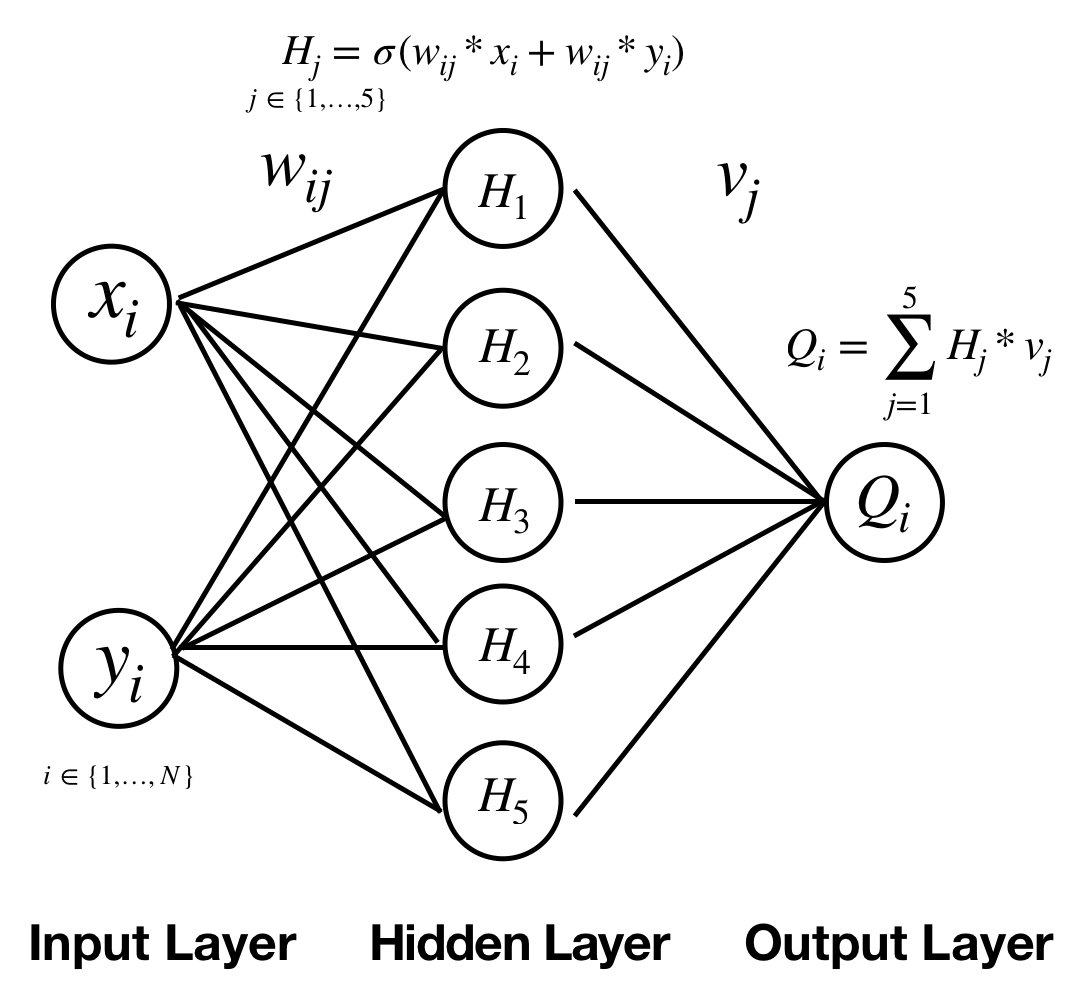
\includegraphics[width=0.4\textwidth]{nn_pde_struct.png}
	\caption{The diagram of Neural Network for computing the parameters of trial solution in pde $O_{i}(x_i,y_i,p)$ with one hidden layer. }
	\label{fig:nn_pde_struct}
\end{figure}
The error quantity to be minimized is given by:
\begin{equation}
E[p] = \sum_{i} \{ \frac{\partial^{2} \Psi (x,y)}{\partial x^2}+ \frac{\partial^{2} \Psi (x,y)}{\partial y^2}-f(x,y)\}^2.
\end{equation}
The form of trial solution is based on the types of Boundary conditions encountered in the solution of partial differential equations. For a Dirichlet BC, the trial solution is:
\begin{equation}
\Psi_{t}(x,y) = A(x,y) + x(1-x)y(1-y)O(x,y,p).
\end{equation}
where $A(x, y)$ is chosen so as to satisfy the BC.
\begin{equation}
A(x, y) = (1-x)f_{0}(y)+xf_{1}(y)+(1−y){g_{0}(x)−[(1−x)g_{0}(0)+xg_{0}(1)]}+y{g_{1}(x)−[(1−x)g_{1}(0)+xg_{1}(1)]}
\end{equation}

\medskip \noindent
where $f_{0}(y)=\Psi_t(0,y)$, $f_{1}(y)=\Psi_t(1,y)$, $g_{0}(x)=\Psi_t(x,0)$ and $g_{1}(x)=\Psi_t(x,1)$.

\medskip \noindent
Figure \ref{fig:nn_pde_struct} illustrate the way to compute the parameters by NN for trial solution in two-dimensional problem. We denote the feedforward function as $O(x,y,p)$.

\medskip \noindent
For a mixed boundary condition, the trial solution is written as:

\begin{equation}
	\Psi_{t}(x,y) = B(x,y) + x(1-x)y[O(x,y,p)-O(x,1,p)-\frac{\partial}{\partial y}O(x,1,p)]
\end{equation}
$B(x, y)$ is again chosen so as to satisfy the BCs.
\begin{equation}
B(x, y) = (1-x)f_{0}(y)+xf_{1}(y)+g_{0}(x)−[(1−x)g_{0}(0)+xg_{0}(1)]+y{g_{1}(x)−[(1−x)g_{1}(0)+xg_{1}(1)]}
\end{equation}

\medskip \noindent
where $f_{0}(y)=\Psi_t(0,y)$, $f_{1}(y)=\Psi_t(1,y)$, $g_{0}(x)=\Psi_t(x,0)$ and $g_{1}(x)=\frac{\partial}{\partial x}\Psi_t(x,1)$.


\section{Convergence Method}

Because we did not apply activation function to the output unit of NN, the value of output does not converge. Therefore, in order to make the output stable, we set the condition that if 
\begin{equation}\label{eq:converge}
| \Psi_t(x_N) - BC| \leq \varepsilon
\end{equation}
\medspace \noindent
and the number of iteration is over 500, then the iteration stops. In (\ref{eq:converge}), we set $BC=\Psi_{a}(x_N)$ and $\varepsilon=e^{-3}$.







\section{Relative Work}

Weinan\cite{weinan} combines backward stochastic differential equation(BSDE) with NN to solve PDE.
Trial solution is for the stochastic control problem.
The stochastic process with continuous sample paths which satisfy that for all $t \in [0,T]$.
\begin{equation}
Y_t = g(\xi + W_T) + \int_{t}^{T}f(Y_s,Z_s)ds - \int_{t}^{T}\langle  Z_s,dW_s \rangle
\end{equation}
The nonlinear PDE is related to BSDE in a sense that for all $t \in [0,T]$ it holds that 
\begin{equation}
Y_t = u(t,\xi + W_t) \in \mathbf{R}, \ \ \ \ Z_t=(\bigtriangledown_{x}u)(t,\xi + W_t) \in \mathbf{R}
\end{equation}
To approximate the trial solution, they can be computed approximately by employing the policy Z.


%\bibliographystyle{unsrt}
%\bibliography{nn_pde}
\begin{thebibliography}{9}
	\bibitem{lagaris}
I. E. Lagaris, A. Likas and D. I. Fotiadis,
\textit{Artifial Neural Networks for Solving Ordinary and Partial Differential Equations},
IEEE Transaction on Neural Networks, vol. 9, No. 5, September 1998

\bibitem{chiaramonte}
M. M. Chiaramonte and M. Kiener,
\textit{Solving differential equations using neural networks}

\bibitem{weinan}
E, Weinan, Han, Jiequn and Jentzen, Arnulf,
\textit{Deep Learning-Based Numerical Methods for High-Dimensional Parabolic Partial Differential Equations and Backward Stochastic Differential Equations},
A. Commun. Math. Stat. (2017) 5: 349.
\end{thebibliography}

\end{document}
